\section{Luthfi Muhammad Nabil (1174035)}
\begin{enumerate}
\item Jelaskan kenapa file suara harus dilakukan MFCC. Dilengkapi dengan ilustrasi atau gambar
Karena MFCC dibutuhkan untuk mengidentifikasi jenis suara. Karena perlunya pengambilan ciri dari suara yang didapat seperti sinyal suara, frekuensi dan gelombang suara untuk dapat diubah menjadi beberapa input lain (Konversi). Karena perlunya komputer untuk mendapat inputan tertentu, maka metode MFCC diperlukan untuk mengkonversi menjadi sesuatu yang dibutuhkan. 
\begin{figure}[H]
    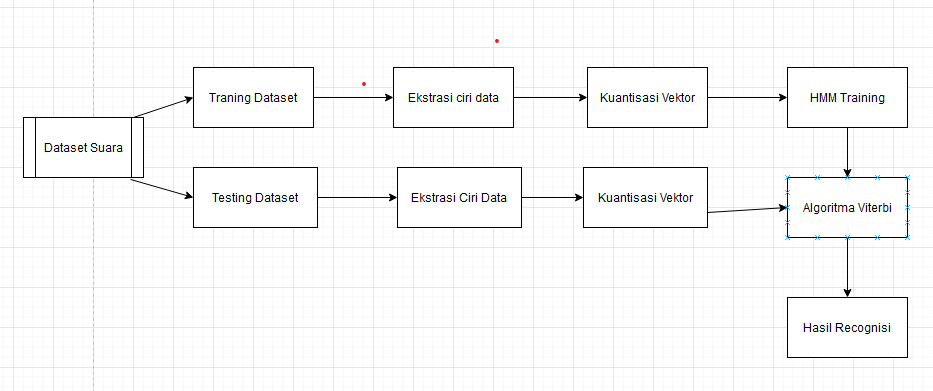
\includegraphics[width=4cm]{figures/1174035/chapter6/teori_1.png}
    \centering
    \caption{Illustrasi MFCC}
\end{figure}
\item Jelaskan konsep dasar neural network. Dilengkapi dengan ilustrasi atau gambar.
Neural Network merupakan kumpulan algoritma yang terinspirasi konsepnya dari otak manusia. Konsep tersebut diantaranya mempelajari pola - pola yang diberikan oleh inputan lain. Untuk menerima data, biasanya Neural Network mendapatkannya dari inputan sensor atau komputasi otomatis yang sudah disediakan oleh programmer untuk melakukan input otomatis ke media Neural Network. Data yang diterima berupa numerik yang terdapat pada vektor yang sesuai dengan data berwujud aslinya. Neural network mengkluster dan menklasifikasikan data untuk dapat disesuaikan dengan parameter - parameter yang sudah ada. 
\begin{figure}[H]
    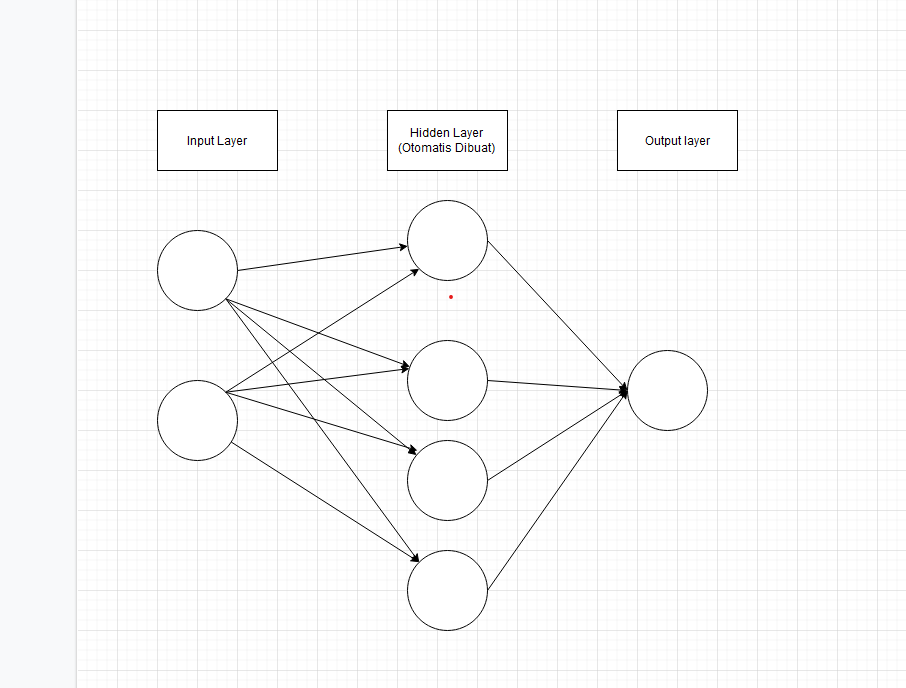
\includegraphics[width=4cm]{figures/1174035/chapter6/teori_2.png}
    \centering
    \caption{Konsep Dasar Neural Network}
\end{figure}
\item Jelaskan konsep pembobotan dalam neural network. Dilengkapi dengan ilustrasi atau gambar
Pembobotan dalam neural network yaitu digunakan untuk membedakan objek inputan atau variabel inputan untuk AI misalkan apel dan jeruk digunakan untuk variabel inputan maka dibuat pembobotan anatara kedua benda tersebut untuk menentukan output yang pasti dari inputan yang dilakukan untuk lebih jelasnya dapat dilihat pada gambar.
\begin{figure}[H]
    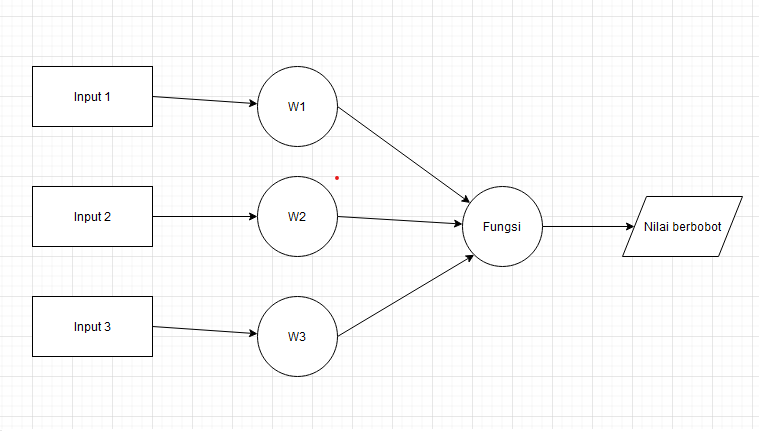
\includegraphics[width=4cm]{figures/1174035/chapter6/teori_3.png}
    \centering
    \caption{Pembobotan Neural Network}
\end{figure}
\item Jelaskan konsep fungsi aktifasi dalam neural network. dilengkapi dengan ilustrasi atau gambar.
Fungsi aktivasi merupakan fungsi yang digunakan untuk mendapatkan output neuron dari nilai inputnya. Fungsi aktivasi akan melakukan penilaian jika output yang dikeluarkan telah mencapai hasil yang telah ditentukan. 
\begin{figure}[H]
    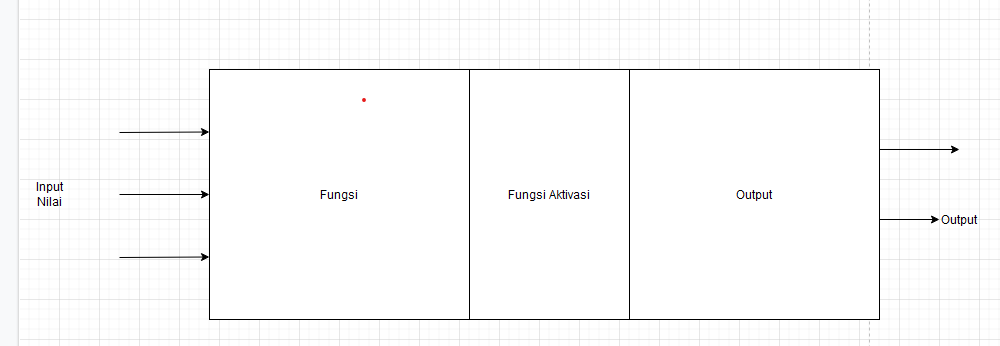
\includegraphics[width=4cm]{figures/1174035/chapter6/teori_4.png}
    \centering
    \caption{Fungsi Aktivasi}
\end{figure}
\item Jelaskan cara membaca hasil plot dari MFCC,dilengkapi dengan ilustrasi atau gambar.
Untuk membaca hasil plotting dari MFCC diantaranya menentukan terlebih dahulu batas minimal gelombang suara (Hz) dan batas maksimal dari suara tersebut. Lalu warna yang paling pekat merupakan hasil dari penglohana data tersebut. Saat membaca file, gelommbang akan diklasifikasikan dengan cara mengkalkulasikan jarak diantara vektor 12 Dimensi. 
\begin{figure}[H]
    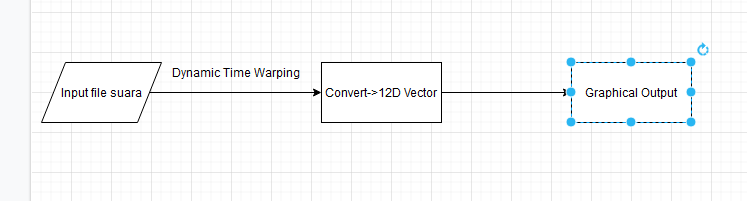
\includegraphics[width=4cm]{figures/1174035/chapter6/teori_5.png}
    \centering
    \caption{Metode pembacaan plot MFCC}
\end{figure}
\item Jelaskan apa itu one-hot encoding,dilengkapi dengan ilustrasi kode dan atau gambar.
One-hot encoding merupakan numerisasi nilai untuk dapat mengindikasikan sebuah status. Karena butuhnya mesin untuk membaca nilai binary, biasanya mesin akan mengkonversi (Decode) terlebih dahulu untuk dapat membaca nilai. Namun saat nilai dilakukan Encoding dengan metode ini, maka nilai tidak perlu di encode lagi karena nilai yang ada sudah merupakan nilai binary. 
\begin{figure}[H]
    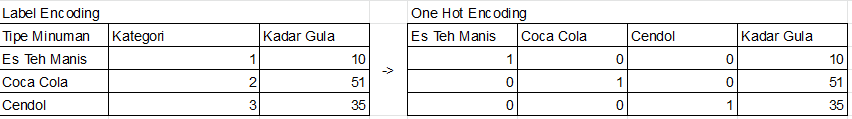
\includegraphics[width=4cm]{figures/1174035/chapter6/teori_6.png}
    \centering
    \caption{One Hot Encoding}
\end{figure}
\item Jelaskan apa fungsi dari np.unique dan to categorical dalam kode program,dilengkapi dengan ilustrasi atau gambar.
Fungsi ini akan mengembalikan array dengan elemen yang berbeda - beda dalam input array. Fungsi ini akan memangkas nilai sehingga hanya beberapa nilai saja yang ada dan nilai tersebut harus berbeda dengan yang lainnya. Biasanya fungsi ini untuk mengidentifikasi jenis nilai atau nilai apa saja yang terdapat pada array yang bersangkutan. to categorical merupakan fungsi untuk mengkonversikan dataset menjadi sebuah beberapa kategori kelas yang ditentukan. Nilai itu sendiri akan diubah menjadi bentuk 'One-hot vector' untuk dapat dibaca oleh komputer.
\begin{verbatim}
    Contoh Program : 
import numpy as np
import keras.utils as ku
arr = [1,5,2,3,3,2,3,3,3,1,2,3,4,5,1,2,5,3,7,8,2,3,7,5,7,2]
print("Awalnya Gini")
print(arr)
#NP Unique akan melepas nilai yang sama
print("Jadinya gini kalau pake np.unique")
print(np.unique(arr))
print("Pakai To Categorical (From keras.utils)")
print(ku.to_categorical(np.unique(arr), num_classes=None))
\end{verbatim}
\begin{figure}[H]
    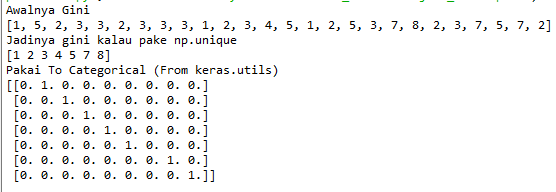
\includegraphics[width=4cm]{figures/1174035/chapter6/teori_7.png}
    \centering
    \caption{Output Contoh program to categorical dan np unique}
\end{figure}
\item Jelaskan apa fungsi dari Sequential dalam kode program,dilengkapi dengan ilustrasi atau gambar.
Sequential berfungsi untuk mencari nilai yang dicari berdasarkan pencarian berurutan sesuai numeric terendah ke tertinggi atau sebaliknya. Sequential dapat digunakan dalam pencarian data vektor untuk mengetahui apakah nilai ada atau tidak. Karena vektor isinya berupa nilai numeric, maka pencarian sequential dapat dijadikan sebagai salah satu metode untuk mencari data tersebut.
\begin{verbatim}
    Contoh Program : 
target = 7
arr = [1,5,2,3,3,2,3,3,3,1,2,3,4,5,1,2,5,3,7,8,2,3,7,5,7,2]
for x in range(0, len(arr)):
if target == arr[x]:
    print("\nNilai "+str(target)+" ada")
    break
\end{verbatim}
\begin{figure}[H]
    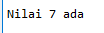
\includegraphics[width=4cm]{figures/1174035/chapter6/teori_8.png}
    \centering
    \caption{Contoh Sequential programming}
\end{figure}
\end{enumerate}
\subsection{Praktek}
\begin{enumerate}
    \item Jelaskan isi dari data GTZAN Genre Collection dan data dari freesound. Buat kode program untuk meload data tersebut untuk digunakan pada MFCC. Jelaskan arti dari setiap baris kode yang dibuat(harus beda dengan teman sekelas).

    \item Jelaskan perbaris kode program dengan kata-kata dan dilengkapi ilustrasi gambar fungsi dari display mfcc() .

    \item Jelaskan perbaris kode program dengan kata-kata dan dilengkapi ilustrasi gambar fungsi dari extract features song(). Jelaskan juga mengapa yang diambil 25.000 baris pertama?

    \item Jelaskan perbaris kode program dengan kata-kata dan dilengkapi ilustrasi gambar fungsi dari generate features and labels().

    \item Jelaskan dengan kata dan praktek kenapa penggunaan fungsi generate features and labels() sangat lama ketika meload dataset genre. Tunjukkan keluarannya dari komputer sendiri dan artikan maksud setiap luaran yang didapatkan.

    \item Jelaskan kenapa harus dilakukan pemisahan data training dan data set sebesar 80 persen? Praktekkan dengan kode dan Tunjukkan keluarannya dari komputer sendiri dan artikan maksud setiap luaran yang didapatkan.

    \item Praktekkan dan jelaskan masing-masing parameter dari fungsi Sequential().Tunjukkan keluarannya dari komputer sendiri dan artikan maksud setiap luaran yang didapatkan.

    \item Praktekkan dan jelaskan masing-masing parameter dari fungsi compile().Tunjukkan keluarannya dengan fungsi summary dari komputer sendiri dan artikan maksud setiap luaran yang didapatkan.

    \item Praktekkan dan jelaskan masing-masing parameter dari fungsi fit().Tunjukkan keluarannya dari komputer sendiri dan artikan maksud setiap luaran yang didapatkan.

    \item Praktekkan dan jelaskan masing-masing parameter dari fungsi evaluate().Tunjukkan keluarannya dari komputer sendiri dan artikan maksud setiap luaran yang didapatkan.

    \item Praktekkan dan jelaskan masing-masing parameter dari fungsi predict().Tunjukkan keluarannya dari komputer sendiri dan artikan maksud setiap luaran yang didapatkan.
\end{enumerate}
\subsection{Praktek}
\begin{enumerate}
    \item Jelaskan isi dari data GTZAN Genre Collection dan data dari freesound. Buat kode program program untuk meload data tersebut untuk digunakan pada MFCC. Jelaskan arti dari perbaris kode yang dibuat (harus beda dengan teman satukelas).\par
    \subitem Isi data data merupakan datasets lagu atau suara yang terdiri dari 10 genre yang di simpan kedalam 10 folder yaitu folder blues, classical, country, disco, hiphop, jazz, metal, pop, reggae, dan rock ke sepuluh folder. Masing - masing dari folder terdapat 100 data suara sedangkan data freesound merupakan contoh data suara yang akan di gunakan untuk menguji hasil pengolahan data tersebut dengan menggunakan metode mfcc. hal tersebut untuk mengetahui apakah suara dari freesound termasuk kategori jazz pop atau sebagainya ?.
    
    \lstinputlisting[firstline=1, lastline=21]{src/1174035/chapter6/chapter6.py}
    \subitem dapat dilihat pada kode diatas pada baris kesatu dilakukan import librosa tang digunakan untuk fungsi mfcc pada suara.
    pada baris kedua dilakukan import librosa featuse dan pada baris ke tiga dilakukan librosa display selanjutnya pada baris ke empat dilakukan import glob kemudian insert numpy untuk pengolahan data menjadi vektor setelah itu dilakukan import matplotlib untuk melakukan ploting setelah itu dilakukan import librari keras.\par
    
    \subitem Selanjutnya yaitu membuat fungsi mfcc dengan nama display mfcc yang didalamnya terdapat variabel y yang berisi method librosa load kemudian variabel mfcc yang berisi method librosa featurea mfcc. Setelah itu membuat plot figure dengan ukuran 10 banding 4 kemudian di isi oleh data librosa display dengan variabel x nya yaitu waktu dan y yaitu mel atau Hz kemudian melakukan plot warna setelah itu melakukan plot judul dan terakhir flot di tampilkan. 
    
    \item Jelaskan perbaris kode program dengan kata-kata dan di lengkapi ilustrasi gambar fungsi dari display mfcc().\par
    
    \lstinputlisting[firstline=22, lastline=43]{src/1174035/chapter6/chapter6.py}
    
    \subitem pada baris ke dua program diatas digunakan untuk mendisplay tampilan glombang suara dari file disco.00067.wav menggunakan metode mfcc dengan menggunakan fungsi display mfcc yang telah tadi di buat pada nomer dua begitu juga pada baris ke 4 6 8 sampai ke 22 secara teksis sama menggunakan fungsi display mfcc hanyasaja beda peyimpanan data yang akan di tampilkan atau di eksekusi. 
    
    \begin{figure}[H]
          \centering
          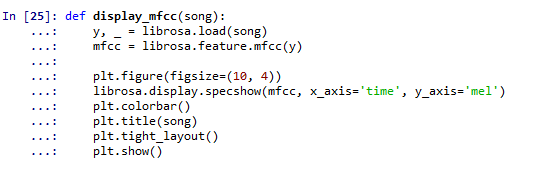
\includegraphics[width=4cm]{figures/1174035/chapter6/praktek_1.png}
          \caption{Ilustrasi gambar fungsi dari displaymfcc() }
          \end{figure}
    
    
    
    \item Jelaskan perbaris dengan kata-kata dan dilengkapi dengan ilustrasi gambar fungsi dari extract features song jelaskan kenapa data yangdiambil merupakan data 25.000 baris pertama ? 
    
    \lstinputlisting[firstline=44, lastline=55]{src/1174035/chapter6/chapter6.py}
    
    \subitem pada baris ke tiga di definisikan nama extract features song yang nantinya akan di gunakan pada fungsi yang lainya kemudian dibuat variabel y dengan method librosa load setelah itu dibuat variabel baru mfcc dengan isi librosa features mfcc dengan isi variabel y tadi kemudian dibuat variabel mfcc dengan isian np.max dan variabel mfcc tadi terakhir di buat array dari data tersebut merupakan data 25000 data pertama. kenapa data 25000 pertama yang digunakan dikarenakan data tersebut digunakan sebagai data testing semakin besar data testing yang di gunakan maka semakin akurat hasil AI. tapi sebenarnya data tersebut relatif bisa lebih besar atau lebih kecil tergantung pada komputer masing masing.
    
    \item Jelaskan Perbaris kode program dengan kata-kata dan di lengkapi ilustrasi gambar fungsi dari generate features and labels.
    
    \lstinputlisting[firstline=56, lastline=76]{src/1174035/chapter6/chapter6.py}
    
    \subitem pada baris ke tiga merupakan pendefinisian nama fungsi yaitu generate features and labels kemudian membuat variabel baru dengan array kosing yaitu all features dan all labels kemudian mendefinisikan isian label untuk gendre dengan cara membuat variabel genres kemudian di isi dengan 10 gendre yang tadi setelah itu dilakukan fungsi if else dengan code for dan in setelah itu akan di buat encoding untuk data tiap tiap label contoh untuk blues 1000000000 dan untuk clasical 0100000000.
    
    \item Jelaskan dengan kata dan praktek kenapa penggunaan fungsi generate features and labels sangat lama saat meload dataset gendre tunjukan keluarannya dari komputer sendiri dan artikan maksud dari luaran tersebut.\par
    
    halnini menjadi lama dikarenakan mesin membaca satupersatu file yang ada pada folder dan dalam foldertersebut terdapat 100 file sehingga wajar menjadi lama ditambah lagi mengolah data yang tadinya suara menjadi bentuk vektor. berikut merupakan codenya.
    \lstinputlisting[firstline=77, lastline=79]{src/1174035/chapter6/chapter6.py}

    
    \begin{figure}[H]
          \centering
          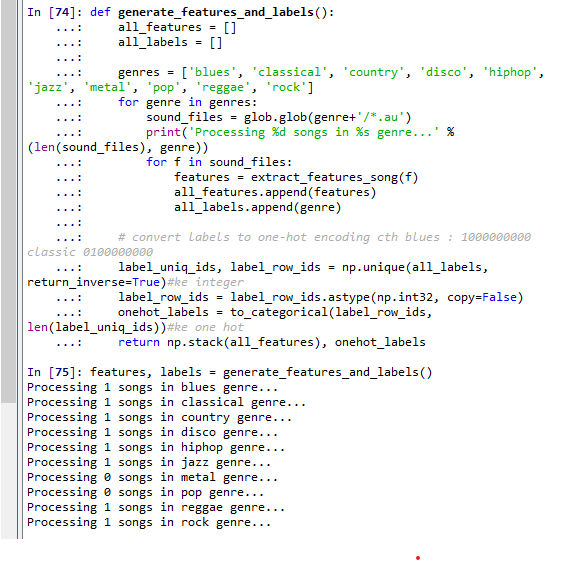
\includegraphics[width=4cm]{figures/1174035/chapter6/praktek_2.png}
          \caption{Hasil dari fungsi generate features and labels}
          
          \end{figure}
    
  
    
    \item jelaskan kenapa harus dilakukan pemisahan data training dan data testing sebesar 80 persen praktekan dengan kode dan tunjukan keluarannya dari komputer sendiri dan artikan maksud dari luaran tersebut. 
    
    untuk code nya adalah sebagai berikut  yang merupakan code untuk membagi data sebanyak 80 persen untuk data training maka data musik tadi yang total jumlahnya 1000 akan di bagi dua untuk data training sebanyak 800  dan 200 untuk data testing.
    
    \lstinputlisting[firstline=83, lastline=84]{src/1174035/chapter6/chapter6.py}
    
 
    \begin{figure}[H]
          \centering
            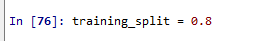
\includegraphics[width=4cm]
          {figures/1174035/chapter6//praktek_3.png}
          \caption{Hasi eksekusi code}
          
          \end{figure}
    
    \begin{figure}[H]
          \centering
          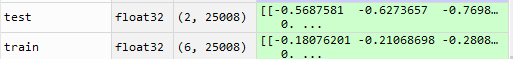
\includegraphics[width=4cm]
          {figures/1174035/chapter6/praktek_4.png}
          \caption{Hasil pembagian 80 persen}
          
          \end{figure}
    
    \item praktekan dan jelaskan masing masing parameter dari fungsi Sequential().  tunjukan keluarannya dari komputer sendiri dan artikan maksud dari luaran tersebut.\par
    \subitem fungsi sequential digunakan untuk mengolah data inputan sesuai dengan fungsi yang ada pada fungsi sequential pada fungsi sequential kali ini menggunakan dua fungsi. fungsi sequential mengkompile data dari 100 neuron atau dari 1 folder file dengan menggunakan fungsi relu dan softmax untuk menghasilkan outputan yang sesuai dengan keriteria.
    \lstinputlisting[firstline=105, lastline=111]{src/1174035/chapter6/chapter6.py}
    
    \begin{figure}[H]
          \centering
          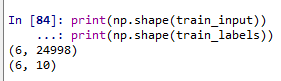
\includegraphics[width=4cm]
          {figures/1174035/chapter6/praktek_5.png}
          \caption{Hasil fungsi sequential}
          
          \end{figure}
    
    \item praktekan dan jelaskan masing masing parameter dari fungsi compile().  tunjukan keluarannya dari komputer sendiri dan artikan maksud dari luaran tersebut. \par
    \subitem yaitu fungsi kompile yang digunakan untuk mengetahui parameter yang digunakan dari data yang telah diolah untuk caranya dapat menggunakan codingan sebagai berikut dan untuk hasilnya akan memunculkan parameternya berapasaja dan total parameter yang digunakan.
    
    \lstinputlisting[firstline=112, lastline=116]{src/1174035/chapter6/chapter6.py}
    
    \begin{figure}[H]
          \centering
          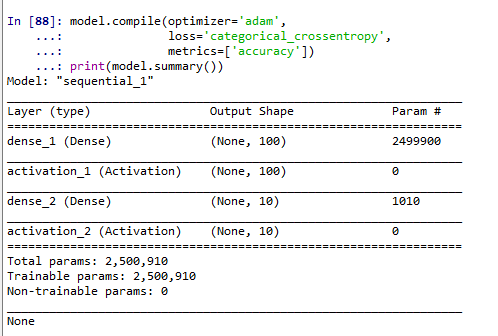
\includegraphics[width=4cm]
          {figures/1174035/chapter6/praktek_6.png}
          \caption{Hasil fungsi compile}
          
          \end{figure}
    
    \item praktekan dan jelaskan masing masing parameter dari fungsi fit().  tunjukan keluarannya dari komputer sendiri dan artikan maksud dari luaran tersebut.\par
    \subitem pada fungsi ini dilakukan pengolahan data dari 10 label tadi atau 10 file data sets tadi kemudian di hitung tingkat akurasi masing masing dan tingkat kegagalan atau loss data darisetiap file tersebut caranya dengan melakukan codingan berikut.data menunjukan 10 pengolahan data untuk menentukan nilai akurasi dan loss dari data tersebut dan selanjutnya dilakukan fingsi evaluasi.
    
    \lstinputlisting[firstline=117, lastline=119]{src/1174035/chapter6/chapter6.py}
    
    \begin{figure}[H]
          \centering
          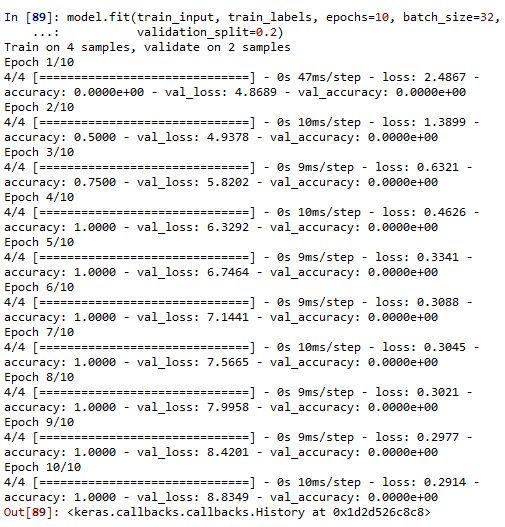
\includegraphics[width=4cm]
          {figures/1174035/chapter6/praktek_7.png}
          \caption{Hasil fungsi fit}
          
          \end{figure}
    
    \item praktekan dan jelaskan masing masing parameter dari fungsi evaluate().  tunjukan keluarannya dari komputer sendiri dan artikan maksud dari luaran tersebut.\par
    \subitem pada fungsi ini dilakukan evaluasi terhadap datayang telah di runing sebelummnya untuk lebih jelasnya dapat di lihat codingan tersebut  pada codingan tersebut dilakukan evaluasi pada tingkat kegagalan dan akurasi kebenaran maka hasilnya akan memunculkan hasil evaluasi dari 10 proses dari setiap gendre yaitu akurasi sebesar 51 persen dan loss data sebesar 1.4105 data.
    
    \lstinputlisting[firstline=120, lastline=125]{src/1174035/chapter6/chapter6.py}
    
    \begin{figure}[H]
          \centering
          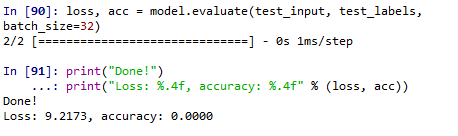
\includegraphics[width=4cm]
          {figures/1174035/chapter6/praktek_8.png}
          \caption{Hasil fungsi evaluasi}
          
          \end{figure}
    
    \item praktekan dan jelaskan masing masing parameter dari fungsi predic  tunjukan keluarannya dari komputer sendiri dan artikan maksud dari luaran tersebut. \par 
    \subitem fungsi predic merupakan fungsi untuk membandingkan tingkat akurasi pada setiap label yang sepuluh tadi maka data akan di sandingkan ke masing masing tingkat akurasinya, yang akurasinya paling tinggi maka itulah jawaban untuk setiap inputan yang dilakukan. 
    
    \lstinputlisting[firstline=126, lastline=127]{src/1174035/chapter6/chapter6.py}
    
    \begin{figure}[H]
          \centering
          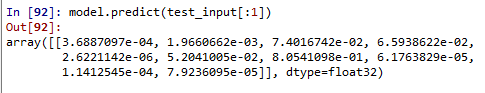
\includegraphics[width=4cm]
          {figures/1174035/chapter6/praktek_9.png}
          \caption{Hasil fungsi prediksi}
          
          \end{figure}
    
    \end{enumerate}

\subsection{Skrinsut error}
\begin{enumerate}
    \item Tipe Error : ValueError
    \item Cara Penanganan : Pastikan array sudah tersedia, karena kasus yang ada disini merupakan kasus pengambilan file, maka cek filenya apakah ada atau tidak
    \begin{verbatim}
        #Before
          sound_files = glob.glob(genre+'/*.sau')
          #after
          sound_files = glob.glob(genre+'/*.au')
          #Note : Tidak ada file .sau di folder, maka diganti ekstensinya
    \end{verbatim}
    \item Skrinsut Error
    \begin{figure}[H]
        \centering
        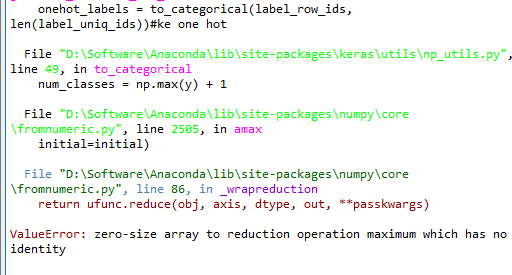
\includegraphics[width=4cm]
        {figures/1174035/chapter6/error.png}
        \caption{Skrinsut error}
        
        \end{figure}
\end{enumerate}